\section{Formal models from figurative language}\label{sec:metaphor}

Figurative language is when language is used non-literally, e.g. \texttt{to bathe in another's affection}. Figurative language subsumes analogy (\texttt{built like a mountain}), metaphor (\texttt{she got a lot out of that lecture}) and some idioms (\texttt{raining cats and dogs}). The issue with figurative language for formal semantics, insofar as formal semantics is concerned with truth-conditions, is that one requires an underlying model in order to begin truth-conditional analysis. The role of figurative language, especially that of metaphor, is in some sense to provide those models in the first place\marginnote{\citep{reddy_conduit_nodate} argues convincingly that the metaphor \texttt{IDEAS are CONTAINERS} is pervasive in English; it is just about the only way we talk about communication. Yet there is no literal sense in which one can 'get something' out of a lecture or 'pack a lot' into a book. Evidently the \emph{systematicity of the metaphor itself} yields the common structure from which we can even begin to consider pedestrian truth-conditional analyses; i.e. language has a role to play in constructing the stage, and afterwards we can reason logically about the actors and events. The process by which language constructs the underlying model is not by nature truth-conditional: there is no fact of the matter before it is read of a fictional character's eye-colour, but it does become a facet of the reader's world-model afterwards. Therefore: of which truth-conditions cannot speak, thereof truth-conditionalists must remain silent.}, so the truth-theoretic (or inquisitive, or dynamic) approach to semantics operates at an inappropriate stage of abstraction. We might illustrate or depict schema to represent figurative language, but to the best of my knowledge, there is no formal account of how the systematicity of a chosen schematic corresponds to the organisation of a metaphor or concept. So what is required is a methodology to construct the underlying models from the figurative language in a more-or-less systematic way.\\

The whole point of mucking around with \textbf{ContRel} earlier is this: figurative language can be formally interpreted as vignettes involving topological figures. I will demonstrate here that cofunctors from \textbf{ContRel} into text-circuits representing utterances are promising candidates for the formalisation of figurative language. My focus will exclude idiomatic language and one-off analogies in favour of metaphor just because the latter is most interesting, though the methodology applies in other cases of figurative language. I will take a \emph{metaphor} to be figurative language that utilises the systematic structure in one conceptual domain to give partial structure in another conceptual domain\marginnote[1cm]{Meta, beyond. Phor, as in amphora, an agent, carrier, or producer. Metaphor carries meaning beyond one domain to another. It bears and produces meaning. Metaphors are the primary agents of meaning.}. This may subsume some cases of what would otherwise be called \emph{similes} or \emph{analogies}. The differences far as I can tell between a metaphor and an analogy is the presence of systematicity in the former, and a weak requirement that the correspondence involves separate conceptual domains. It doesn't really matter for this discussion what the difference is.\\

First, we observe that we can model certain kinds of analogies between conceptual spaces by considering structure-preserving maps between them. For example, Planck's law gives a partial continuous function from part of the positive reals measuring tempature of a black body in Kelvin to wavelengths of light emitted, and the restriction of this mapping to the visible spectrum gives the so-called "colour temperature" framework used by colourists. It will turn out that a decategorified cofunctor has the right kind of structure.\\

Second, we observe that we can use simple natural language to describe conceptual spaces, instead of geometric or topological models. Back to the example of colour temperature, instead of precise values in Kelvin, we may instead speak of landmark regions that represent both temperature and colour such as \texttt{incandescent} and \texttt{daylight}, which obey both temperature-relations (e.g. \texttt{incandescent is cooler than daylight} and colour-relations (e.g. \texttt{daylight is bluer than incandescent}).\\

Third, we observe that we can also use simple natural language to describe more complex conceptual schemes with interacting agents, roles, objects, and abilities. This will require a cofunctor. Organising this linguistic data in the concrete structure of a text circuit allows us to formally specify what it means for one conceptual scheme to structure another by describing structure-preserving maps between the text circuits. This will allow us construct topological models of metaphors such as \texttt{TIME is MONEY}.\\

Finally, I will describe a preliminary taxonomy of different kinds of metaphor, and discuss what is to be done.

\subsection{Temperature and colour: the Planckian Locus}

\begin{example}[The Physicists' Planckian Locus]\label{ex:planck1}
Planck's law describes the spectral radiation intensity of an idealised incandescent black body as a function of light frequency and temperature. Integrating over light frequencies in the visible spectrum yields a function from temperature of the black body to chromaticity.
\begin{figure}[h]
\centering
\scalebox{0.5}{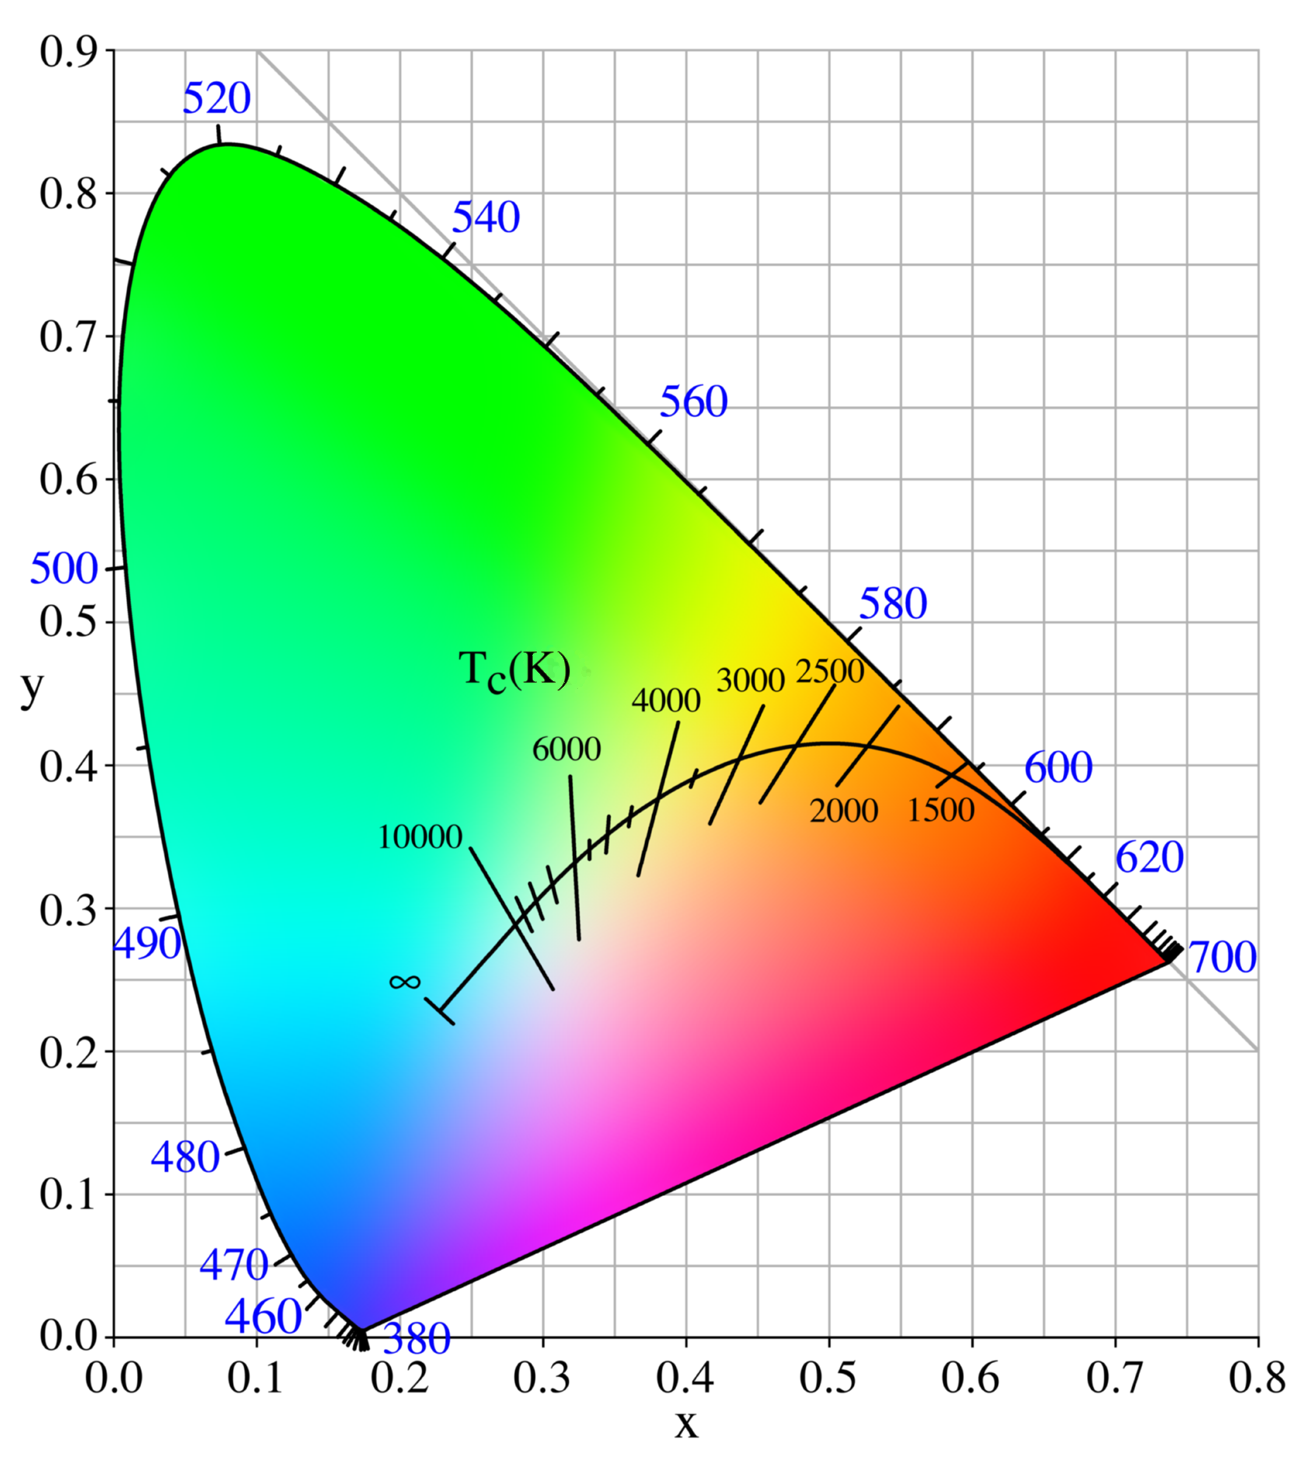
\includegraphics{figures/metaphor/PlanckianLocus}}
\caption{The Planckian Locus in the CIE 1931 chromaticity diagram. Chromaticity refers only to the hue of a colour, without other domains such as saturation.}
\end{figure}
\end{example}

Abstractly, the Planckian Locus is a continuous function mapping the positive real line representing the conceptual domain of temperature into the plane representing the conceptual domain of colour. The Planckian locus is the basis of colourist-talk about colour schemes in terms of temperature, which allows them to coordinate movements in colourspace using the terminology of temperaturespace, e.g. \texttt{make this shot warmer}. This fits with what we would prototypically expect a metaphor to allow us to do with meanings.

However, the particular mathematical conception of metaphor-as-map in Example \ref{ex:planck1} is too rigid: it only goes one way. It is a specific and inflexible kind of metaphor that does not behave at all outside its specified boundaries. For example, colourists have to deal with offsets towards green and magenta, which are not in the chromaticity codomain of the function given by Planck's law. It would be truer to life if we further analysed the function as mediated by a strip.

\begin{example}[The colourist's Planckian Locus]
Now we aim to extend our mathematical model to accommodate the fact that colourists deal with chromatic offsets or deviations from the mathematically precise locus given by Planck's law.
\begin{figure}[h]
\centering
\scalebox{0.5}{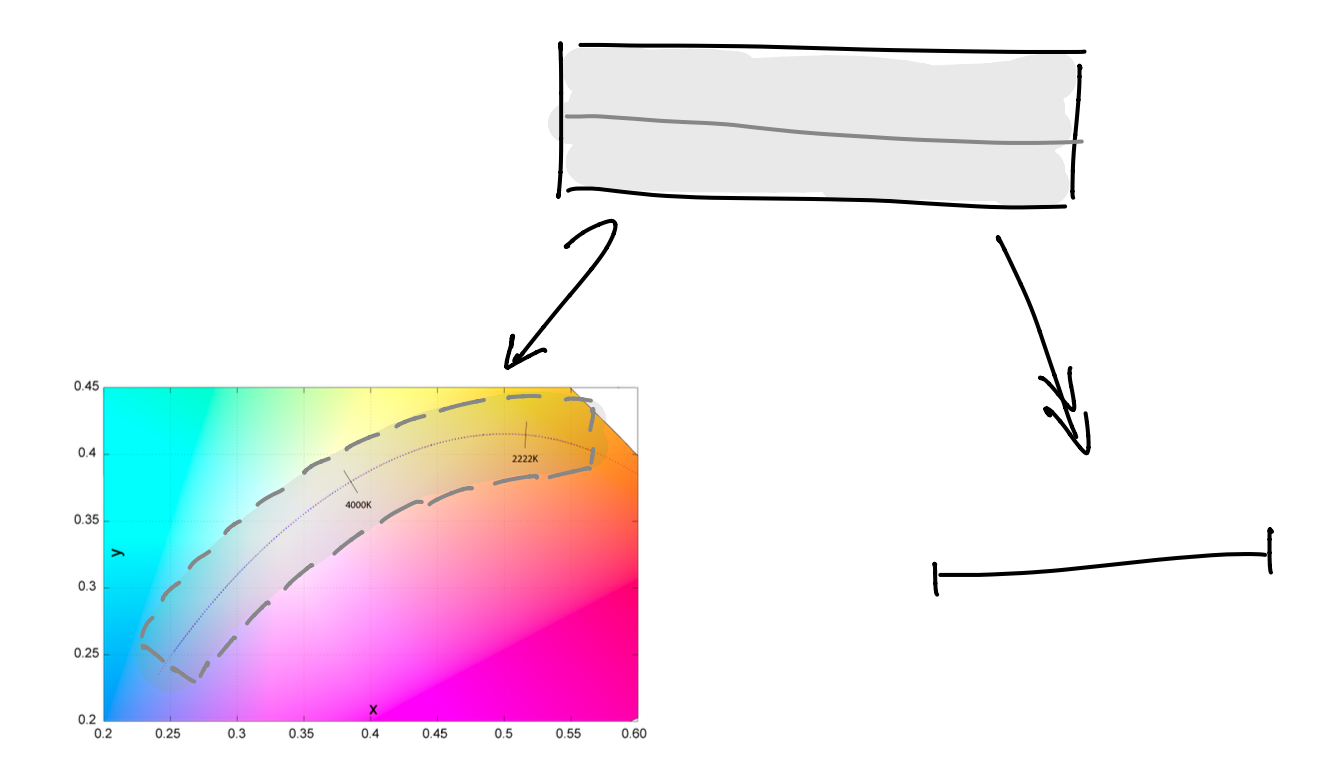
\includegraphics{figures/metaphor/colourlocus1}}
\caption{Consider the unit square (depicted as a strip) as a fiber bundle over the unit interval representing temperature range. There is an injective continuous map from the strip into colourspace that is centered on the Planck Locus.}
\end{figure}
\begin{figure}[h]
\centering
\scalebox{0.5}{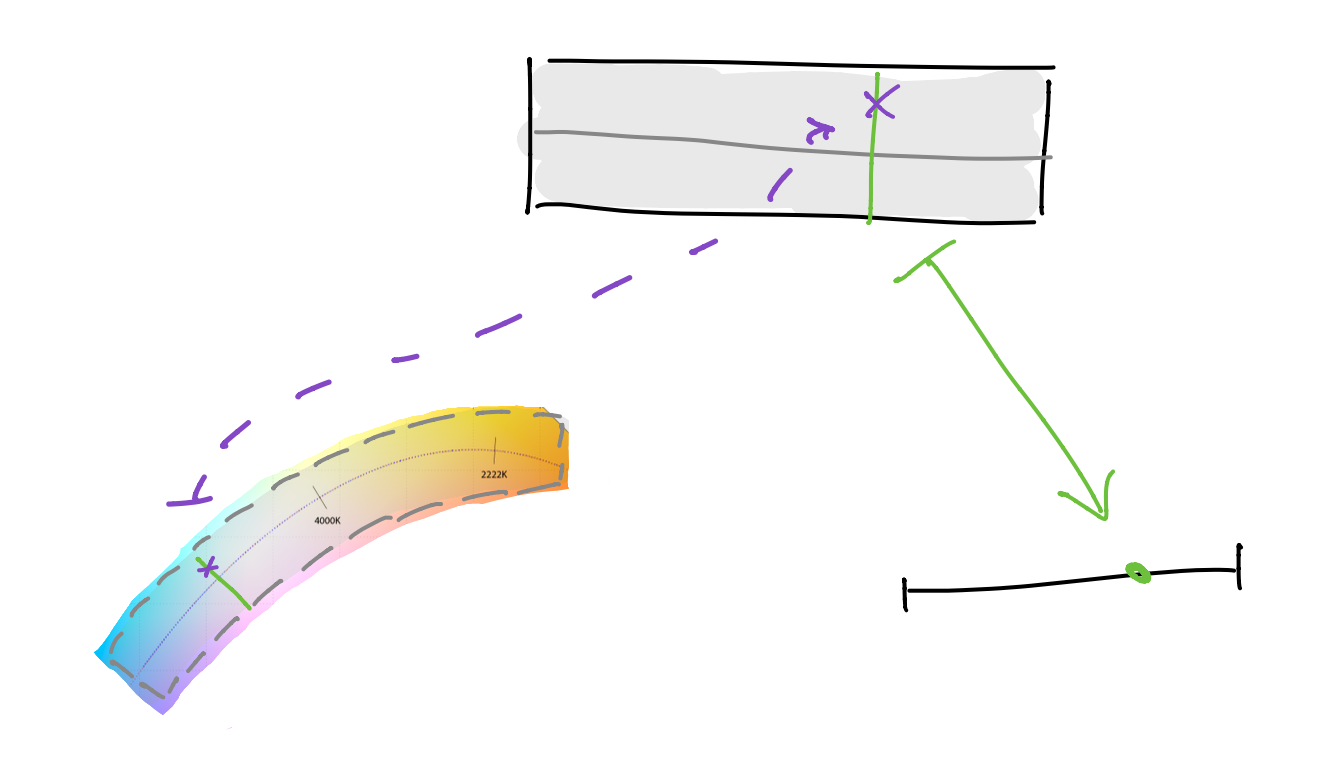
\includegraphics{figures/metaphor/colourlocus2}}
\caption{The left leg is bijective in the image restriction, so any point or displacement in the offset-strip in colourspace can be lifted to a point in the apex strip, which is then projected down along with other points in the vertical fiber to a point in temperaturespace. So we have a decategorified cofunctor!}
\end{figure}
\end{example}

A refinement we have just captured is the partially-structuring nature of metaphor \citep{lakoff_metaphors_2003}. In the language of our running example, pure green is outside the scope of the colour-temperature correspondence given by the Planckian Locus, so the metaphor is only a partial structuring of the colour domain according to the temperature domain. This partiality in the colour domain means that it would have been inappropriate to model the passage of colour-talk to temperature-talk as a function from colour to temperature, as functions are total, rather than partial, on their domain. While it is conceptually nice that we are on the way to recovering monoidal cofunctors as a model of metaphor, why didn't we stay simple and just use a partial function? The answer is that the strip at the apex represents the \emph{talk} part of colour- and temperature-talk.

\begin{example}[Conceptual transfer between domains]
When colourists use the temperature metaphor they might say "hot", "warm", "cooler", which are not specific temperature ranges in Kelvin, but concepts in temperature-space. Recalling that we may consider concepts to be open sets of a topology (and comparatives as opens of the product), we observe that we can linguistically model regions on the positive reals with words \texttt{little} (labelled $l$), \texttt{lot} (labelled $L$), and \texttt{more} (labelled $M$), an algebraic basis from which derive \texttt{less} by symmetry, and other regions such as \texttt{more than a little, less than a lot}. In this particular running example, it happens that both legs of the span of functors have a lifting property, which explains how we might model the fact that conceptual colourist-talk of "daylight" or "candlelight" in the colour domain can be sensibly interpreted in the temperature domain. The formalisation of this fact follows by symmetry from this example.
\begin{figure}[h]
\centering
\resizebox{0.8\textwidth}{!}{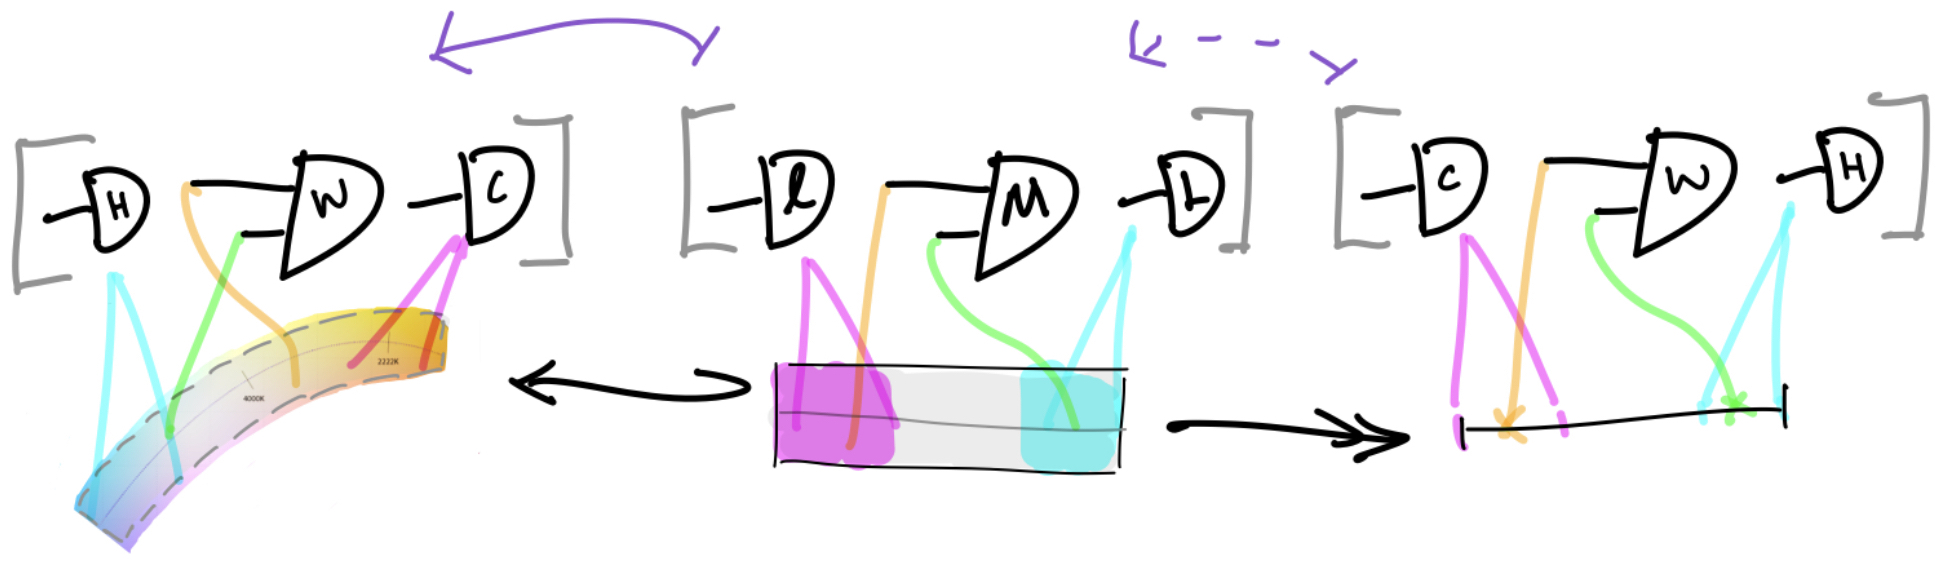
\includegraphics{figures/metaphor/offset1.jpeg}}
\caption{Starting from the right, the lifting property of the right leg is what lets us map "hotter and colder" temperature talk into the more abstract quantity-talk of "more and less" in the apex strip. Then the left functor sends quantity-talk into the colour domain, which allows "hotter and colder" to be used in the colour domain.}
\end{figure}
\begin{figure}[h]
\centering
\resizebox{0.8\textwidth}{!}{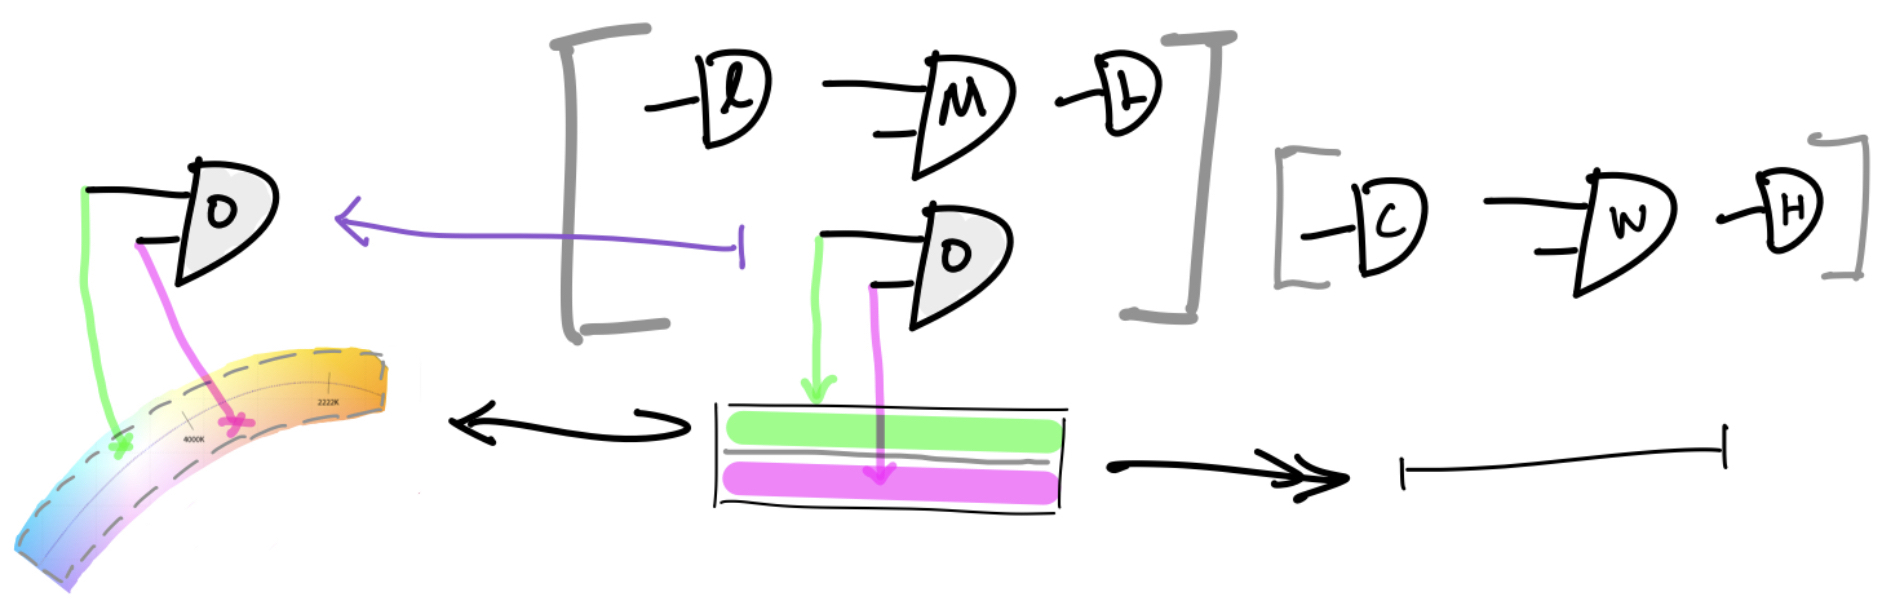
\includegraphics{figures/metaphor/offset2.jpeg}}
\caption{The additional expressive power that the apex strip gives is the concept of vertical offset, which doesn't appear in the real line. So the apex strip allows talk of quantity and offset, and this offset, when translated into the colour domain, allows talk of offset towards and away from, for instance, green.}
\end{figure}
\end{example}
\clearpage

\subsection{Time and Money: complex conceptual structure}

Metaphor is perhaps the only methodology we have for making sense of certain abstract concepts, such as Time. For example, many languages make use of the metaphor \texttt{TIME is SPACE}, in which space-talk is used to structure time. In English, the future is ahead of us and the past behind, while conversely, for the Aymara the future is behind and the past is ahead. Orthogonally, in Mandarin the future is below and the past is above. We have already demonstrated that we have the tools to deal with conceptual transfer between static conceptual spaces viewed as topological spaces via spans of continuous maps. What is of concern to us are \emph{dynamic} metaphors that involve a conceptual space-\emph{time} with agents and capabilities and so on. The following discussion draws heavily from \citep{lakoff_metaphors_2003}.\\

For example, in English, we make ample use\footnote{To our detriment. We could just as well have chosen the metaphor \texttt{TIME is FOOD}, which provides a liberating sense of mastery (at least in a context where food is abundant): time can be prepared, produced, consumed, spiced if dull and best shared with loved ones.} of the metaphor \texttt{TIME is MONEY}. There two mathematically relevant aspects of metaphor that I want to draw attention to for this metaphor. Firstly, that the conceptual affordances money-talk is marshalled to give structure to time-talk, where there is no such structure were it not for the metaphor. Secondly, that metaphor has a partial nature, in that it is not the case that the metaphor licenses all kinds of money-talk to structure time-talk.\\

To establish the first point of conceptual transfer, a phrase like \texttt{Do you have time to look at this?} is completely sensible to us, but literally meaningless; even if we had an oracle to measure possession, what would we point it at to measure a person's possession of time? Even if we accept some argument that the concept of possession is innate to the human faculty, when we say \texttt{This is definitely worth your time!} or \texttt{What a waste of time.}, we are drawing upon value-talk that is properly contingent in the socially constructed sense upon the conceptual complex of money.\\

To establish the second point of partiality, consider that money can be stored in a bank, whereas there is no real corresponding thing in the common conceptual vocabulary which one can store time and withdraw it for later use\footnote{Although, in a wonderful example of `pataphysical thinking, "Time Banks" have existed since the 19th century, which are practices of reciprocal service exchange that use units of time as currency.}. But the partiality constraint is itself partial. For instance, one can invest money into an enterprise in the expectation of greater returns, and this is not appropriate for many domains of time-talk, but there is a metaphorical match in some specific contexts, such as text-editor-talk: \texttt{learning vim slows you down at first but it will save you time later}.\\

Now I'll try to demonstrate by example that the kinda-cofunctors we explored in Section \ref{sec:miracle} between text circuits do all of the things we have asked for. The components of text circuits serve as an algebraic basis for dynamic conceptual complexes, while the kinda-cofunctor handles partial structuring of one conceptual domain in terms of another.

\begin{example}[\texttt{Vincent spends his morning writing}]
To begin a formal figurative interpretation via the metaphor \texttt{TIME is MONEY}, we require some model of the conceptual domain of money, as well as a topological interpretation. As a first pass, we understand that money can be exchanged for goods and services, so we will settle for a text-circuit signature for trade to serve as the conceptual domain as the apex of a cofunctor, given in Figure \ref{fig:tradesig}. The elements of the topological model are given in Figure \ref{fig:topmodel}. The behaviour of the fibration part of the cofunctor is detailed in Figure \ref{fig:fibroles}, and that of the identity-on-objects functor in Figures \ref{fig:interpret}, \ref{fig:time0}, and \ref{fig:time1}. The figurative model serves as a foundation from which truth-theoretical semantics can begin. In the sketched interpretation, there aren't too many interesting questions one can ask, but the purpose of this example is to point out that in principle, we can exploit the systematicity of metaphor by constructing figurative mechanical models for which interesting questions can be asked and answered truth-theoretically, as in Figure \ref{fig:fullermodel}.
\begin{figure}[h]\label{fig:tradesig}
\centering
\resizebox{\textwidth}{!}{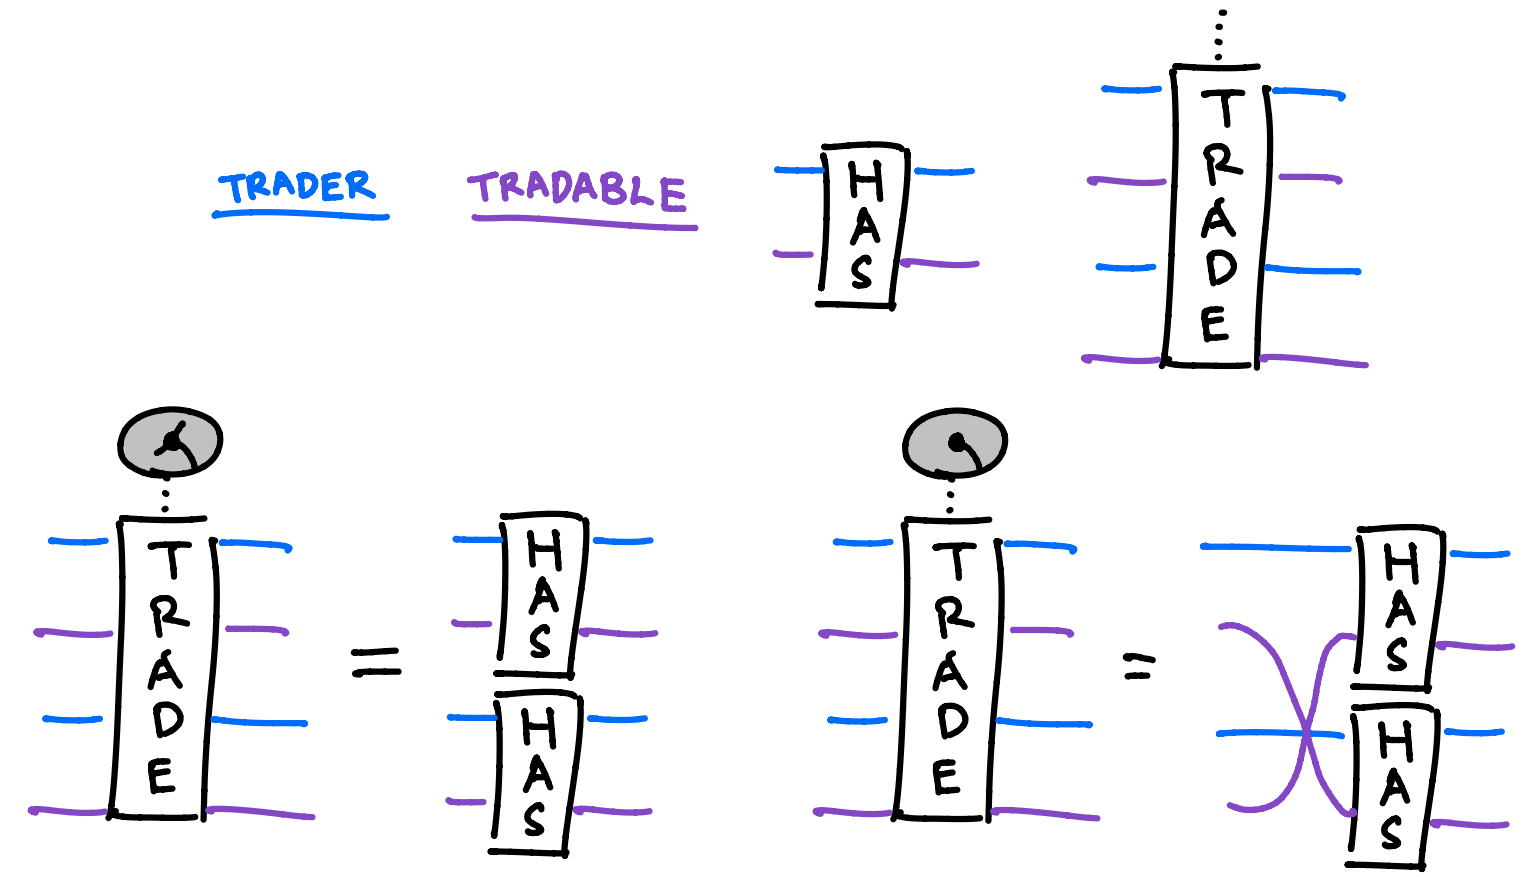
\includegraphics{figures/metaphor/tradesignature}}
\caption{In the \texttt{TRADE} signature, we define two roles as wires: \texttt{TRADERS} and \texttt{TRADEABLES}. There is one static relation \texttt{HAS} to indicate a trader's ownership of a tradeable, which can be further elaborated with equations to indicate e.g. exclusivity of ownership by interpreting violations of exclusivity as a zero morphism, assumed but elided for brevity. There is one dynamic verb (treated as a homotopy) \texttt{TRADE}, which at time 0 enforces a precondition that the traders have their respective tradables, and at time 1 (completion of the trade), the traders swap possession of their tradeables. The \texttt{TRADE} signature contains all nominal instantiations of nouns with respect to roles, which will be illustrated shortly.}
\end{figure}
\begin{figure}[h]\label{fig:topmodel}
\centering
\resizebox{0.75\textwidth}{!}{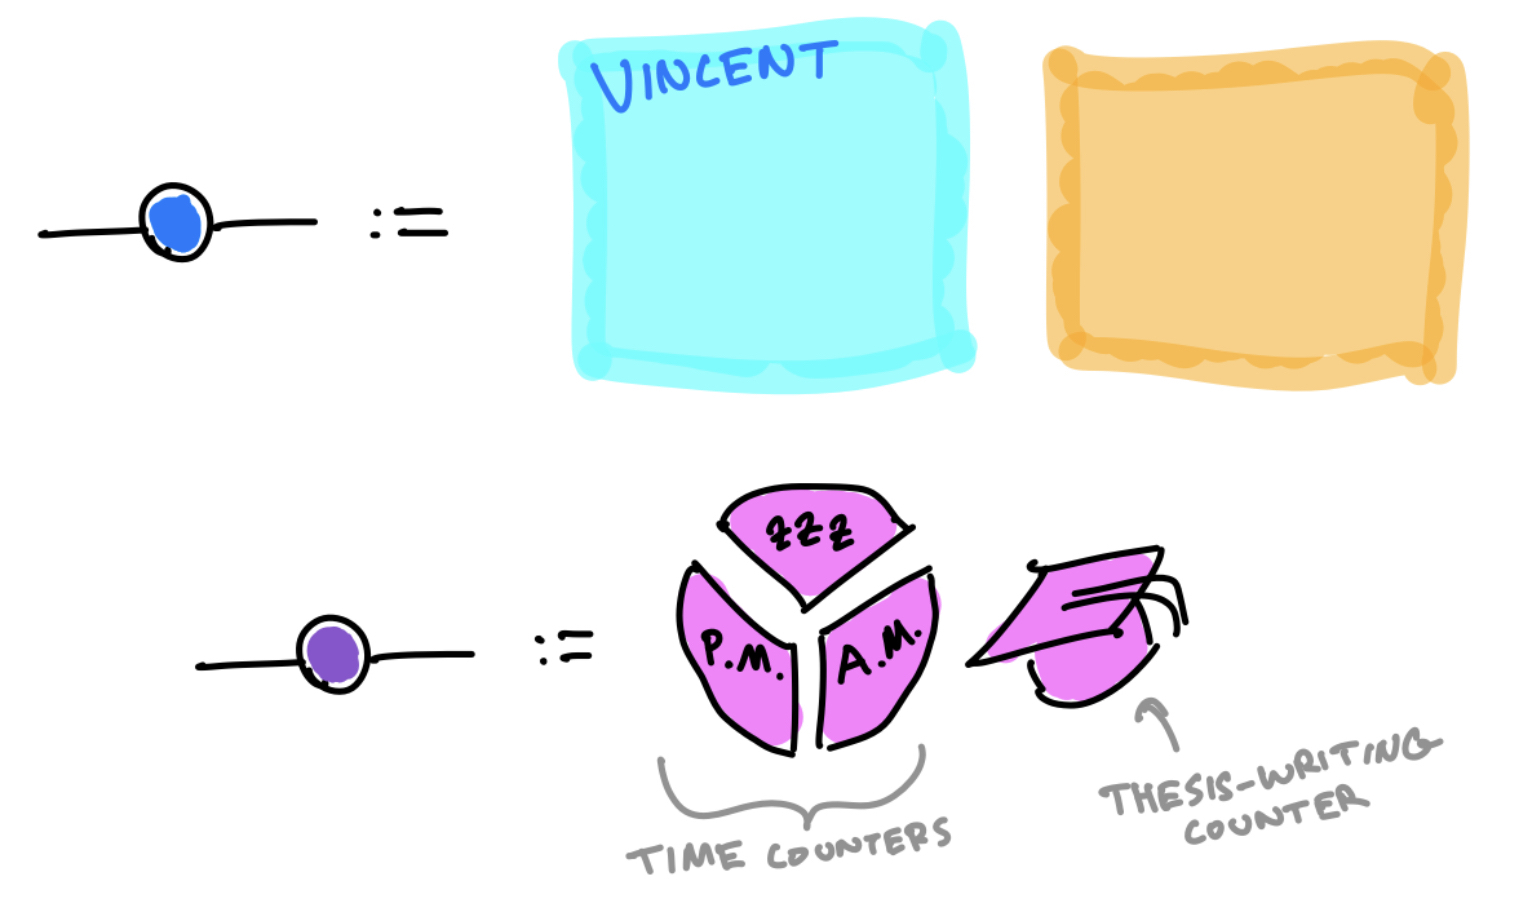
\includegraphics{figures/metaphor/toptrademodel.jpeg}}
\caption{We build the topological model from two sticky spiders in the Euclidean plane. The \texttt{TRADER} spider will distinguish two regions of possession, so that \texttt{HAS} may be interpreted as a region-test. The \texttt{TRADEABLES} spider will specify four meeples or counters, three for time, and one for thesiswriting; we will use the configuration space of the \texttt{TRADEABLES} spider to regulate their movement and distribution.}
\end{figure}
\begin{figure}\label{fig:fibroles}
\centering
\resizebox{\textwidth}{!}{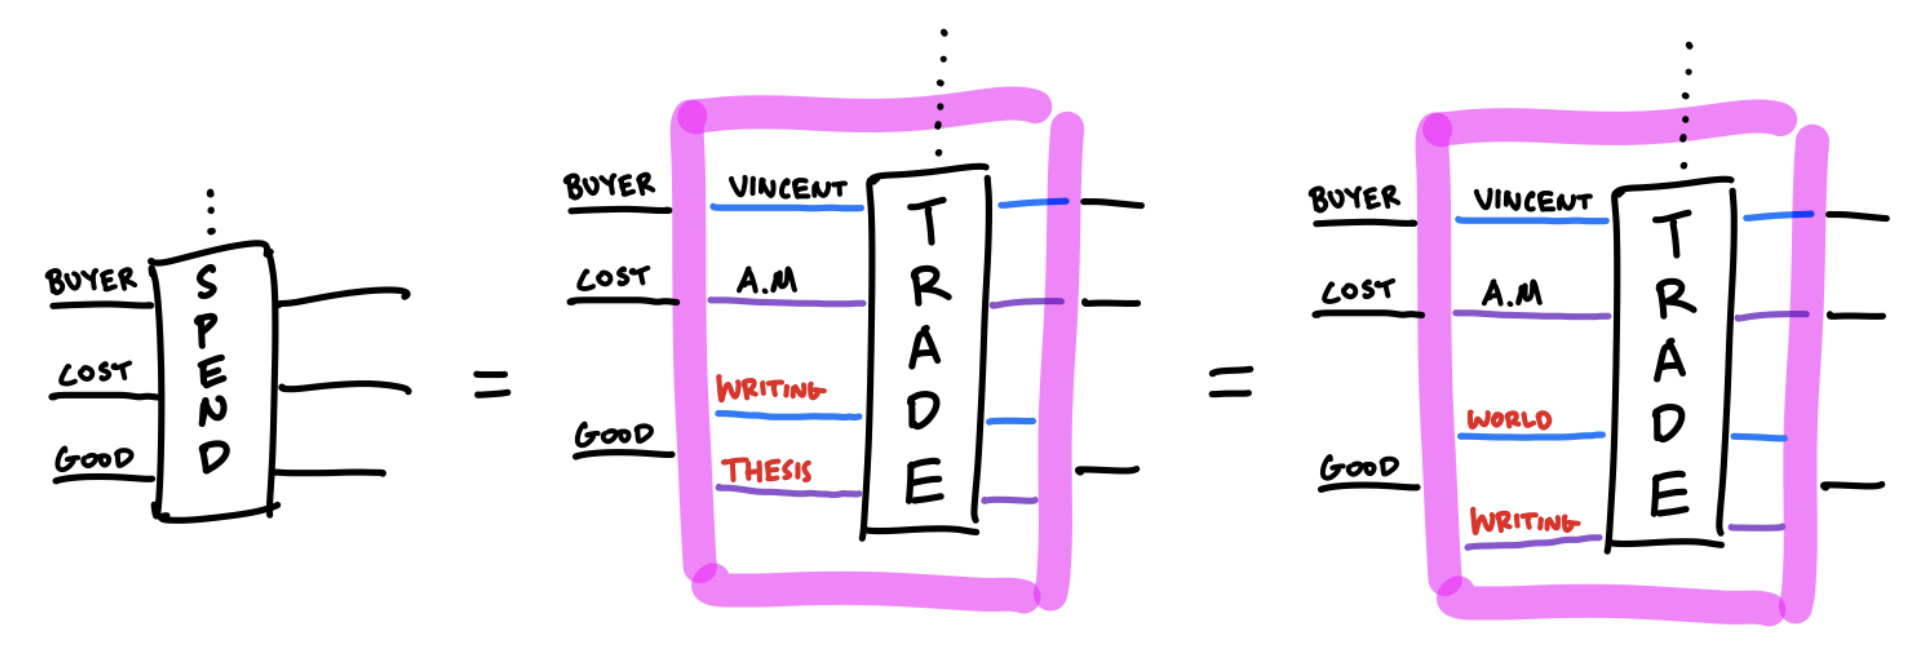
\includegraphics{figures/metaphor/fibroles}}
\caption[-10cm]{Next, we have to specify what the discrete opfibration is doing. Recalling our functor box notation, we can consider the job of the discrete fibration to be role assignment from the verb \texttt{SPEND} in the utterance to the verb \texttt{TRADE} in the conceptual domain. The fibration forgets about role-assignments in its domain by sending them to the monoidal unit. The lift of the fibration is a role-assignment. (Arguably) unambiguously in this example, \texttt{Vincent} is the spender and the first trader, and \texttt{A.M} is the cost and the first tradeable. However, there are two options to resolve \texttt{writing} treated as a noun-phrase in the role of \texttt{GOOD}. In the first lift, \texttt{writing} is resolved as the other trader, and the implicit good as \texttt{thesis}. In the second lift, \texttt{writing} is the tradeable and something else is the trading counterparty, such as \texttt{the world}.}
\end{figure}
\begin{figure}[h]\label{fig:interpret}
\centering
\resizebox{0.5\textwidth}{!}{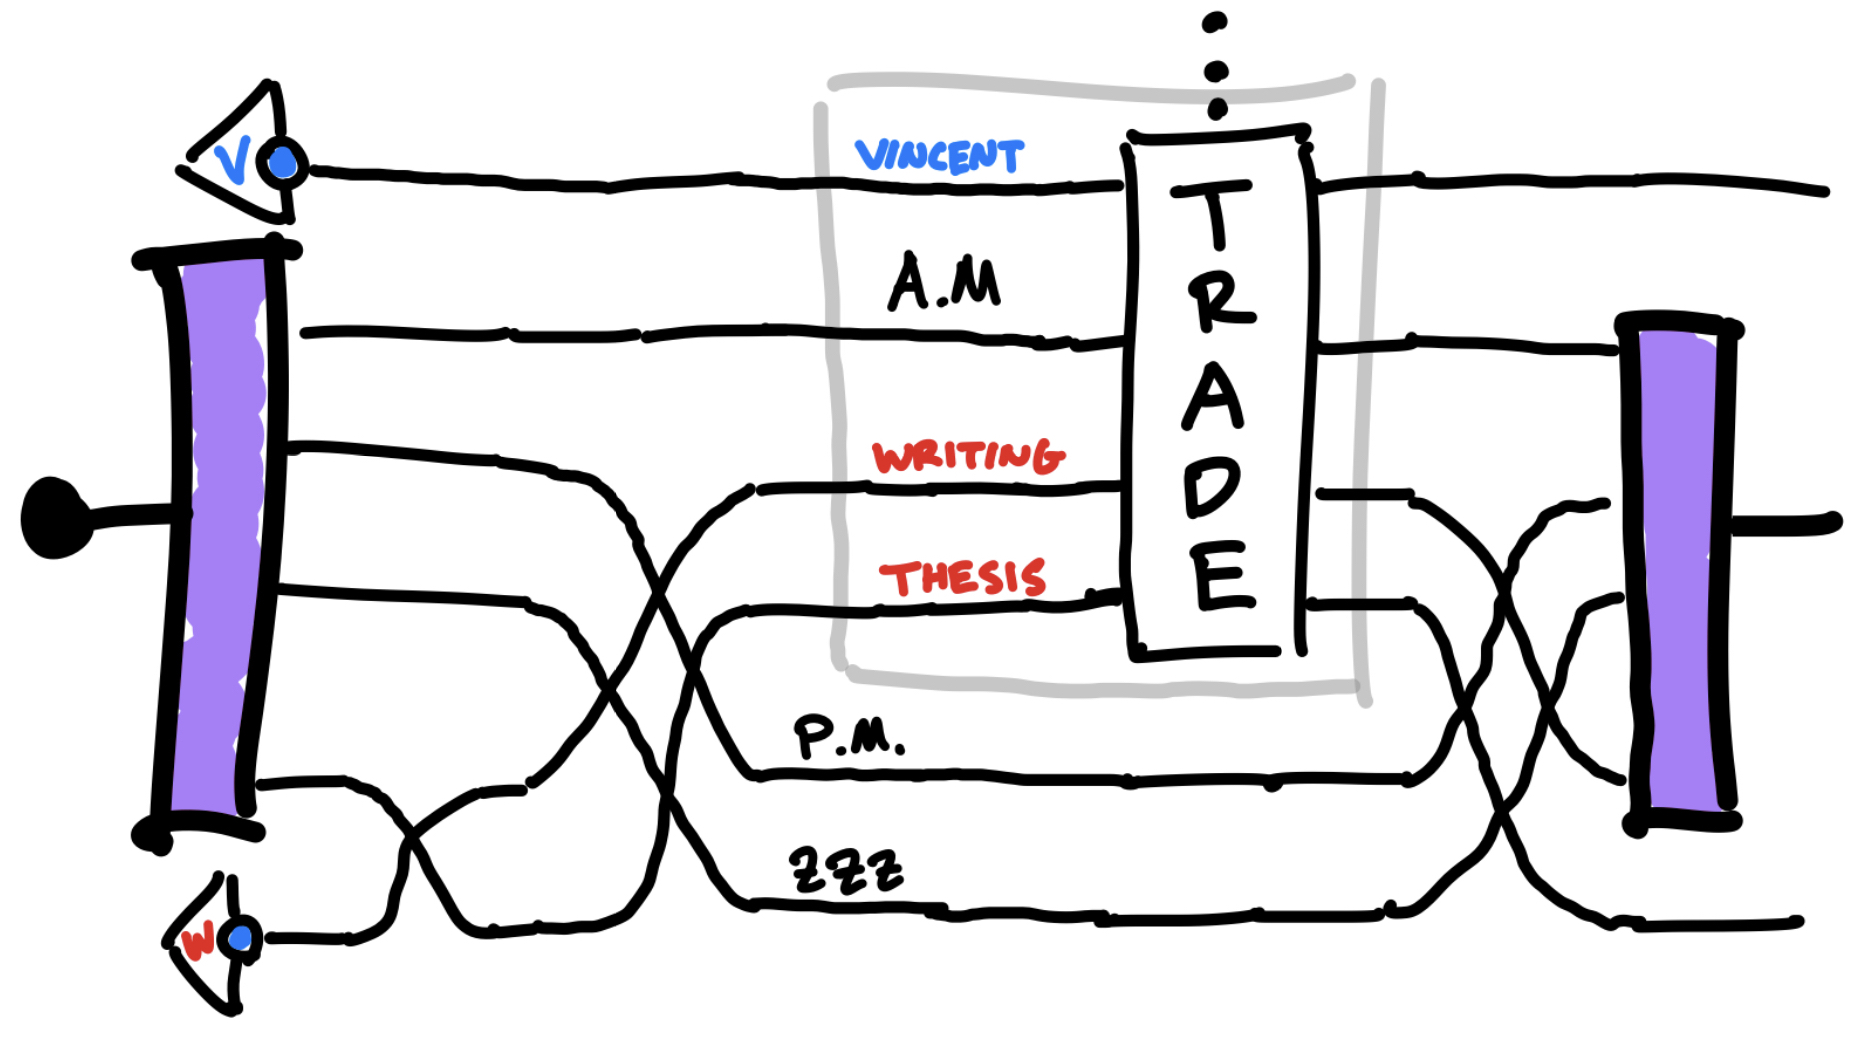
\includegraphics{figures/metaphor/interpret.jpeg}}
\caption{The section of the fibration over the \texttt{SPEND} verb is a tabulation of all the ways in which conceptual roles in the \texttt{TRADING} domain can be assigned. To continue the example, we will assume the first lift in Example \ref{fig:fibroles} as our interpretation. The identity-on-objects functor part of the cofunctor maps our chosen interpretation into the following diagram in \textbf{ContRel}. The configuration space of the \texttt{TRADEABLES} spider is expanded via split idempotent so that all thin wires in the diagram are typed as the Euclidean plane. Recalling Example \ref{ex:chessboard}, \texttt{HAS} is interpreted as the intersection of the position of a counter with the possessive region of the respective trader.}
\end{figure}
\begin{figure}[h]\label{fig:time0}
\centering
\resizebox{\textwidth}{!}{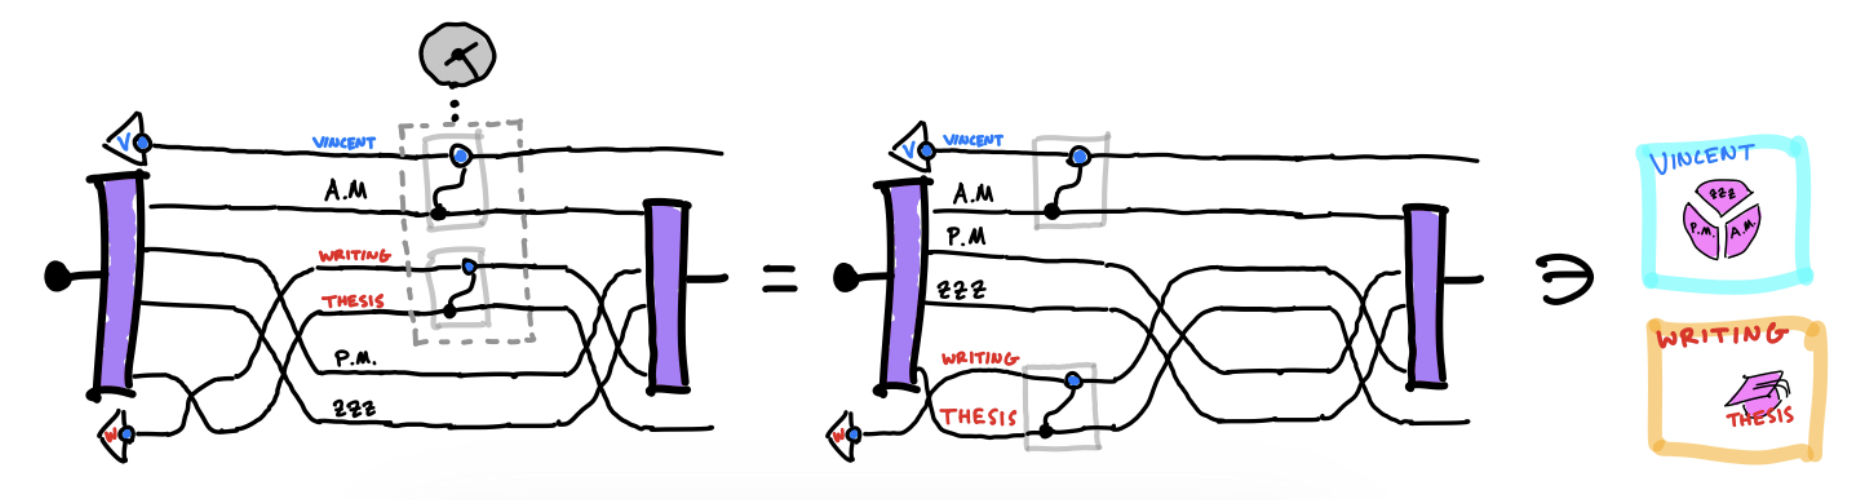
\includegraphics{figures/metaphor/time0.jpeg}}
\vspace{5cm}
\caption{We may verify that the equations governing \texttt{TRADE} cohere with our topological figures. At time 0, before the trade, we can calculate that the permissible figures have \texttt{Vincent} in possession of \texttt{A.M} and \texttt{writing} in possession of \texttt{thesis}.}
\end{figure}
\begin{figure}[h]\label{fig:time1}
\centering
\resizebox{\textwidth}{!}{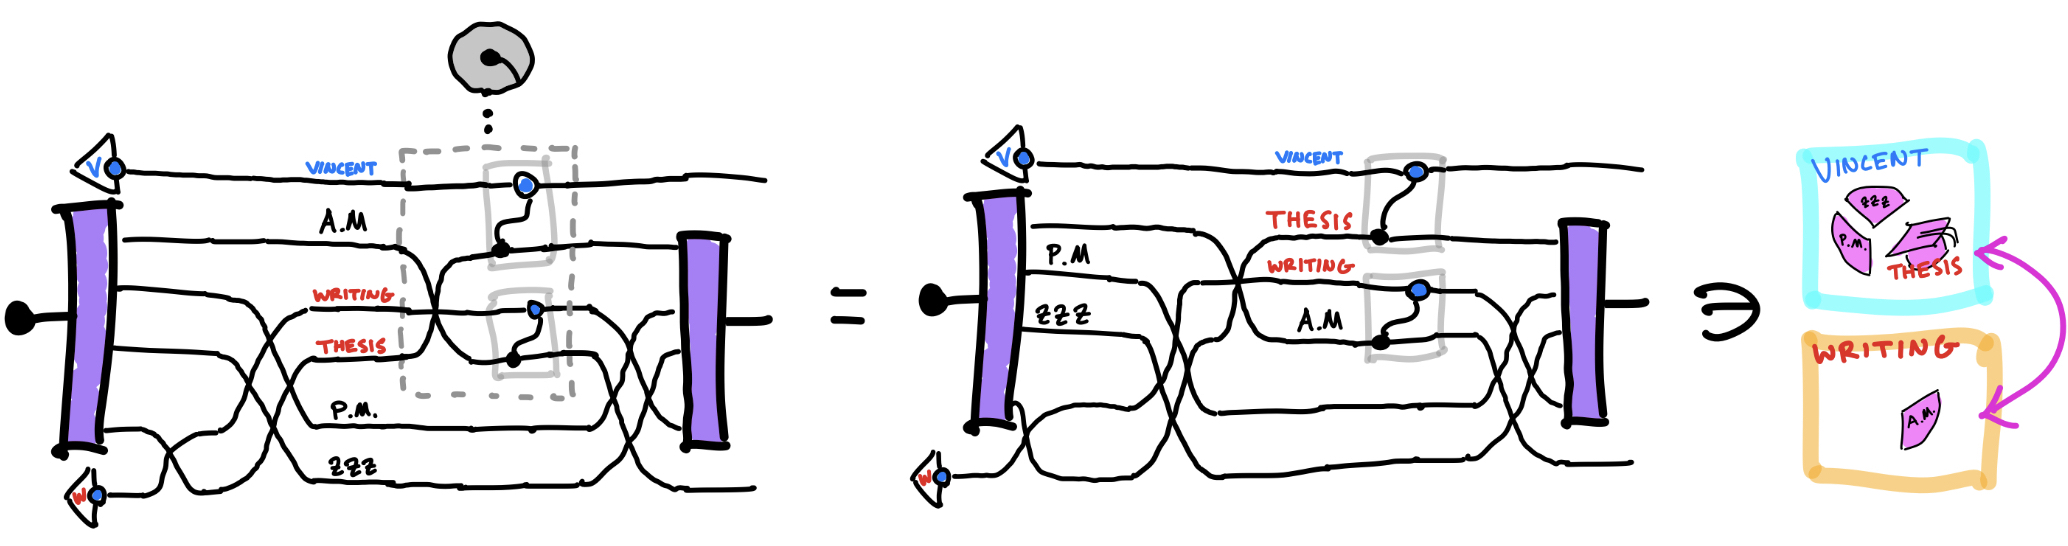
\includegraphics{figures/metaphor/time1.jpeg}}
\caption{At time 1, we may calculate that the permissible figures must be such that \texttt{Vincent} is in possession of \texttt{thesis} and \texttt{writing} is in possession of what was previously my morning.}
\end{figure}
\begin{figure}[h]\label{fig:fullermodel}
\centering
\resizebox{\textwidth}{!}{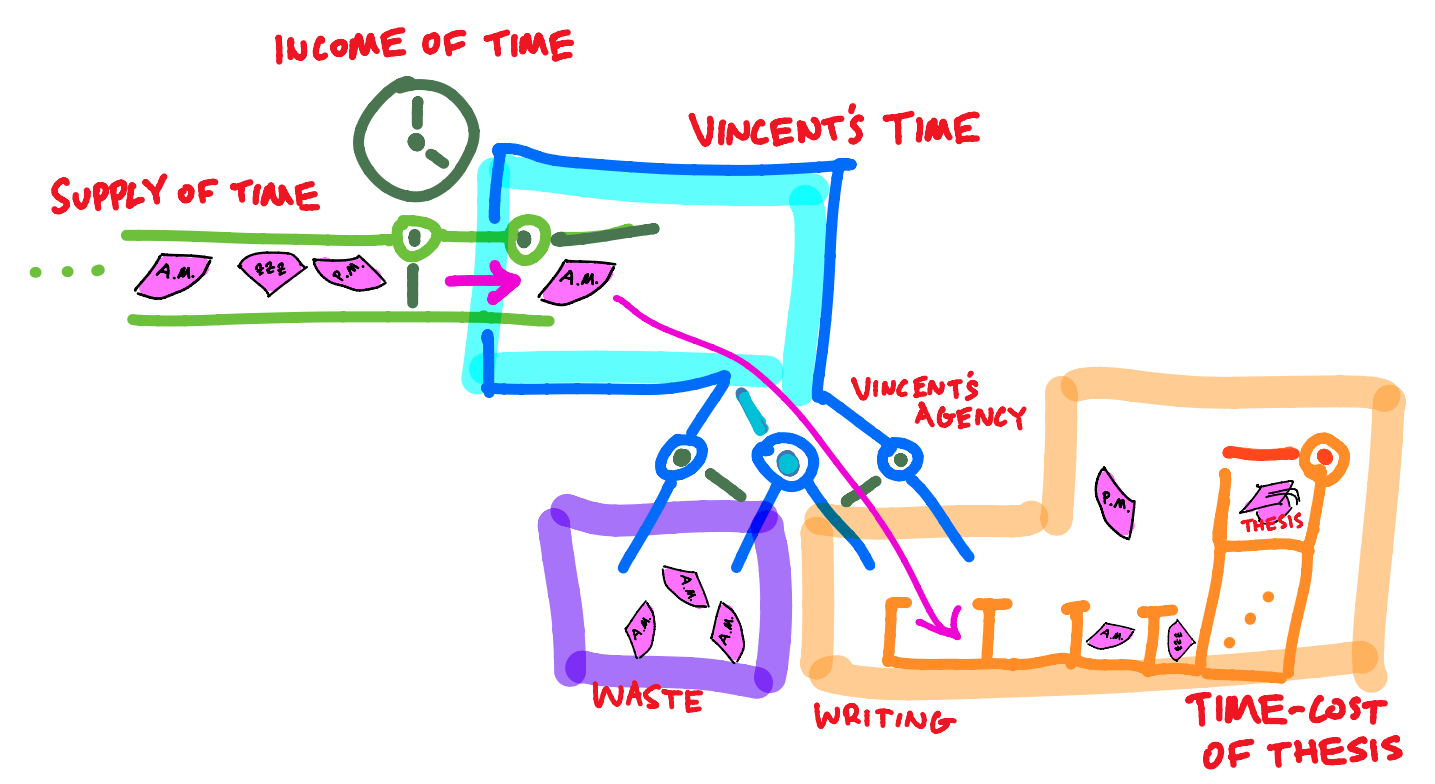
\includegraphics{figures/metaphor/fullermodel}}
\caption{In a more detailed conceptual model of \texttt{TIME is MONEY}, rather than just \texttt{TRADE}, we might consider income, the spender's agency, and cost. In Euclidean 3-space, we might model income as a clock-gated mechanism that deposits time-tokens serially into Vincent's possession, along with his agency as a gated chute, and the time cost of writing a thesis as a dispenser that requires a certain number of tokens to release a thesis-token into Vincent's possession. In this sketch model, one obtains short films for \texttt{He used to waste his mornings but now he spends them writing}, or \texttt{He once spent an evening writing but made no progress}. One can then ascertain certain consequences truth-theoretically; for instance that there is at least one morning that was not spent on writing, or that there is at least one evening spent on writing but not inside the slot that would help a thesis-release mechanism trigger. In every case, cofunctoriality handles bookkeeping for role-interpretation choices and guarantees systematicity of the topological figure according to the signature at the apex model that models the organising concept.}
\end{figure}
\end{example}

\clearpage

\clearpage
\newpage

\newthought{\textbf{Objection:} Hold on, that last figure wasn't justified.} It's justified in principle.

\newthought{\textbf{Objection:} On what principles?} Good question!

\section{The logical conclusions}

Like how the Church-Turing thesis is a declaration of the limits of computability by informed consensus, we might ask what idealised theses we might posit. Now we recap what we've seen.

\newthought{Review of Chapter 1.} We demonstrated that by encoding meaning-relations as topological connectivity (which is in a broad sense the whole point of string diagrams as a bridge between algebra and topology), we can capture systematic structural relationships as configurations of functors. In particular, we were able to diagrammatically reason about the correspondence between a pair of simple productive and parsing grammars subject to the evident constraints of communication. With some imagination, there are two theses here to obtain, or declare:

\begin{thesis}[String diagrams for composition]
Compositionality equals topological representability; in particular, meaning relations in text are witnessed by connectivity of string diagrams.
\end{thesis}

\begin{thesis}[String diagrams for systematic relationships]
Systematicity equals functorially witnessed relations; in particular, spans of functors between families of string diagrams witness agreement between different theories as topological equivalence.
\end{thesis}

\newthought{Review of Chapter 2.} We demonstrated that from the  mathematical perspective of weak $n$-categories, there is no fundamental difference between a broad class of productive grammars at a structural level, including all string-rewrite systems, tree-adjoining grammars, and transformational grammars. In this setting, we created a circuit-growing grammar and demonstrated a correspondence -- the Text Circuit Theorem -- between text circuits and grammatical text for a fragment of English, hence justifying the na\"{i}ve composition of text circuits as a generative grammar. We moreover indicated how the correspondence could be expanded to cover larger fragments of English, and indicated how the particular form of text circuits made them preferable for practical application. We also mentioned that in some sense the correspondence wasn't important from the perspective that text circuits were algebraic jazz for text. Putting together the views from Chapters 0, 1 and 2, productive grammars are just ways of generating topological data, and the only practically interesting constraint about whether a productive grammar is suitable for natural language stems from whether it is paired with a parsing grammar that systematically agrees on semantics up to topological equivalence -- i.e. precisely the kind of equivalence that string diagrams are invariant under. So we might reach for:

\begin{thesis}[String diagrams for syntax]
Syntax equals a coherent method of synthesising \emph{and} analysing composition; in particular, any internally consistent conception of natural language syntax in terms of string diagrams is permissible.
\end{thesis}

\newthought{Review of Chapter 3.} We give content to string diagrams by interpreting them in the category of continuous relations \textbf{ContRel}. We string-diagrammatically characterised labelled collections of disjoint shapes, along with processes that allowed us to puppeteer them in space, and test for topological relationships between shapes and places such as containment and touching. In particular, since we defined rigid motions and spatial-exclusivity of shapes, we have covered enough to linguistically specify any mechanical model up to topological invariance, and it is no difficulty to see how this setting may be expanded to include distances, directions, and forces. We saw how \textbf{ContRel} naturally gives voice to the structure of text circuits as higher-order modifications, and we also saw how \textbf{ContRel} permits us to model simple intensions via containers that mirror the space around them, which also yields a novel mathematical model of \textbf{FinRel} equipped with a Turing object, which is a mathematical model for universal computation and, in the linguistic setting, syntactic polymorphism. On the faith that any consistent and interesting system of string diagrams has some consistent and interesting computational reification, we might integrate the views of the previous chapters to obtain:

\begin{thesis}[String diagrams for semantics]
Semantics equals computatation; in particular, any consistent computational interpretation of the content of string diagrams is permissible.
\end{thesis}

\subsection{How things could be.}

\begin{thesis}[String diagrams for text]
String diagrams suffice for formal linguistics.
\end{thesis}

That's the best-case scenario if we accept all of the best-case scenarios above. What would such a hypothetical world look like? Recall that I still owe a worked example of computing a metaphor. Sadly, I think in a best-case hypothetical world, working out the conduit metaphor would be a kind of dull problem sheet for undergraduate mathematical linguists, who may well ask "what's the point?". Indeed, what is the point of learning all of this mathematically complicated machinery to do something everyone can do effortlessly? I'm not sure of the answer, but I do know that turning language into pictures by turning language into pictures was good fun.

\newpage

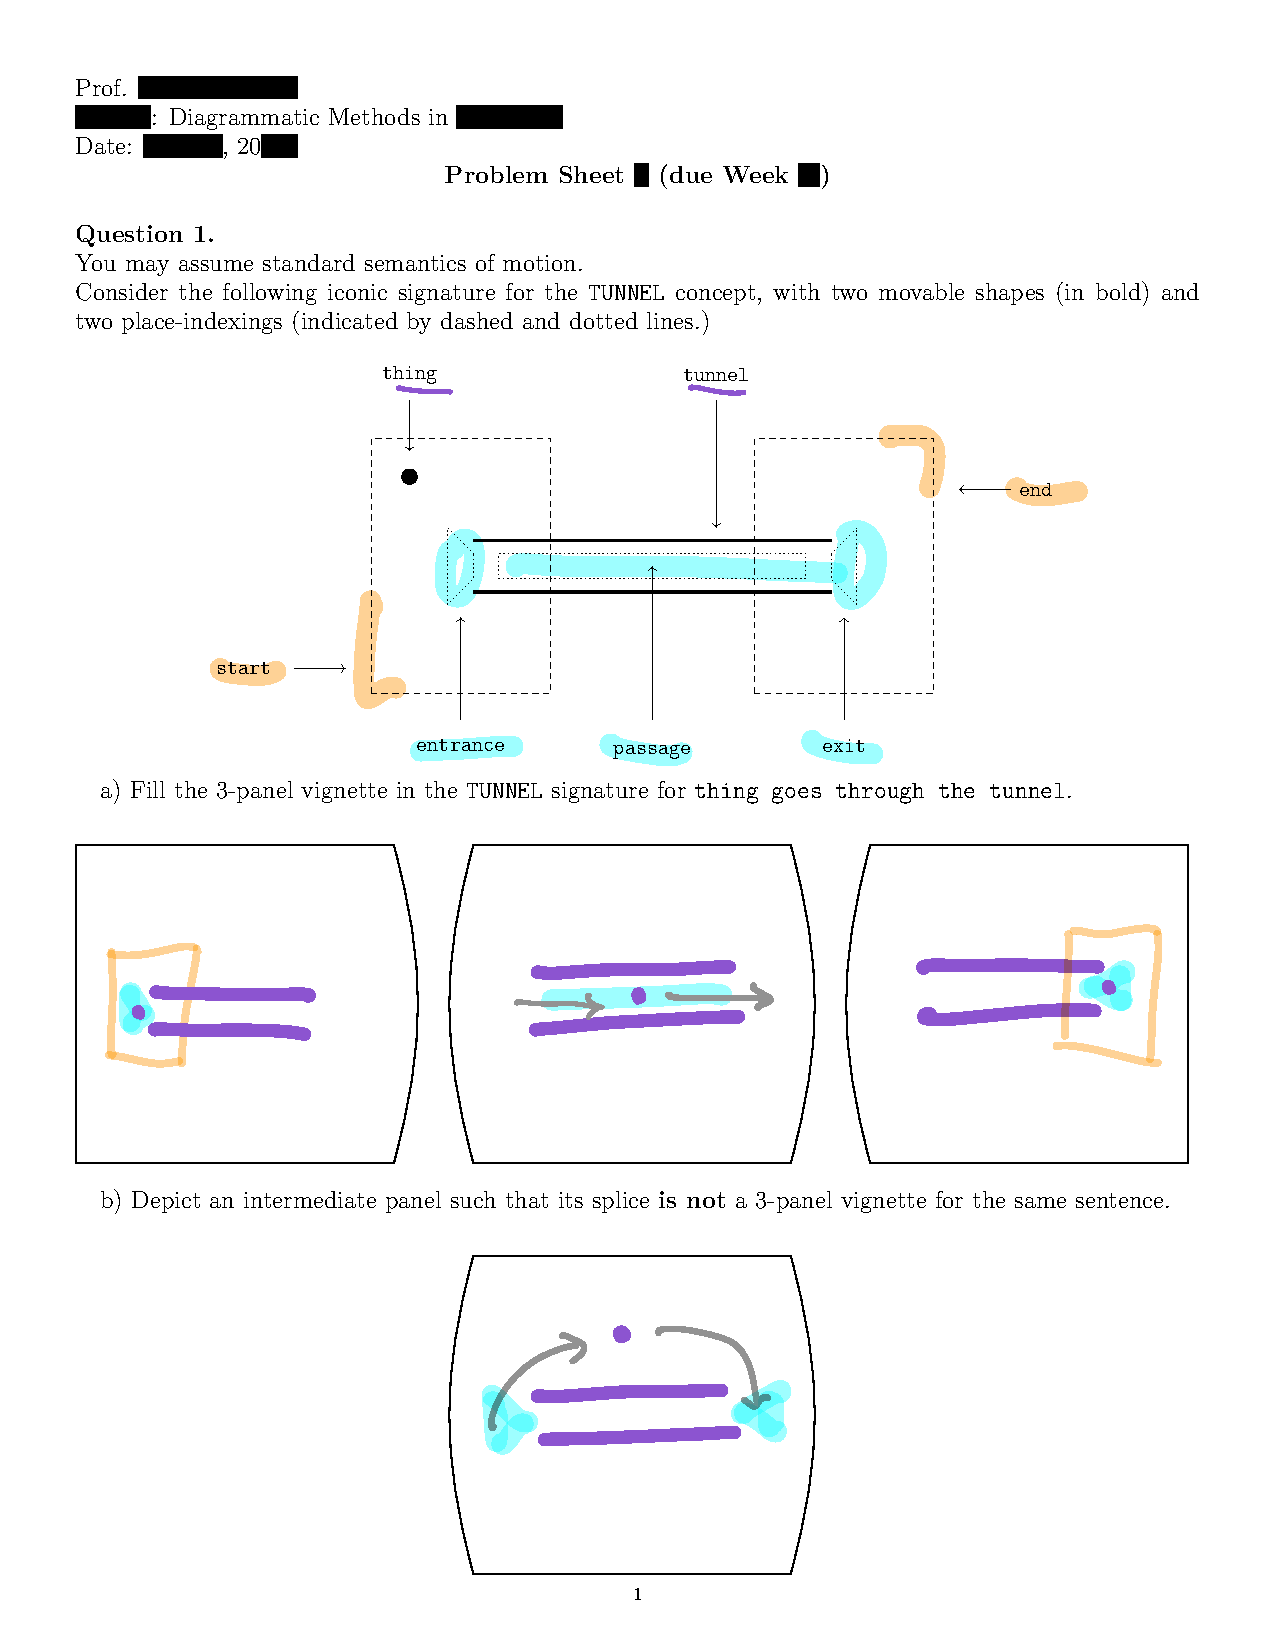
\includepdf[angle=90,pages=-]{metaphorproblemsheet-filled}